\section{Introduction}

Model-Driven Software Development focuses on managing domain-specific models, which represent concerns at conceptual level. Those models are generally represented as various artefacts, in many languages and representations. Model-Driven approach also generally requires code generators, which allow to generate source code. Underlying semantics of code to be executed in generally encoded in those code generators and can be inlined or implicitly defined by code generation process, or may be sometimes explicit to the code generation. Figure \ref{fig:ClassicalVision} shows the classical vision for for Model-Driven Engineering.

A first major drawback of this approach is the gap created between the conceptual level (the model) and the source code, where semantics may be totally hidden or implicit. Another classical issue resides in the development or maintenance process, where model and source code must evolve independently (and sometimes by different actors, eg architect and developer). Round-tripping mechanisms are commonly used to overcome those difficulties, but those tools are difficult to use and maintain, and the process may lead to inextricable issues in a context of concurrent modifications of model  and source code. For those reasons, major software developments projects abandon the idea of maintaining the link between model and source code during development process. In that context, the model is developed at the early stages of development process, and is used to prototype software application. The model may be manually reviewed back at the end of development process, for documentation purposes.

\begin{figure}
    \centering
    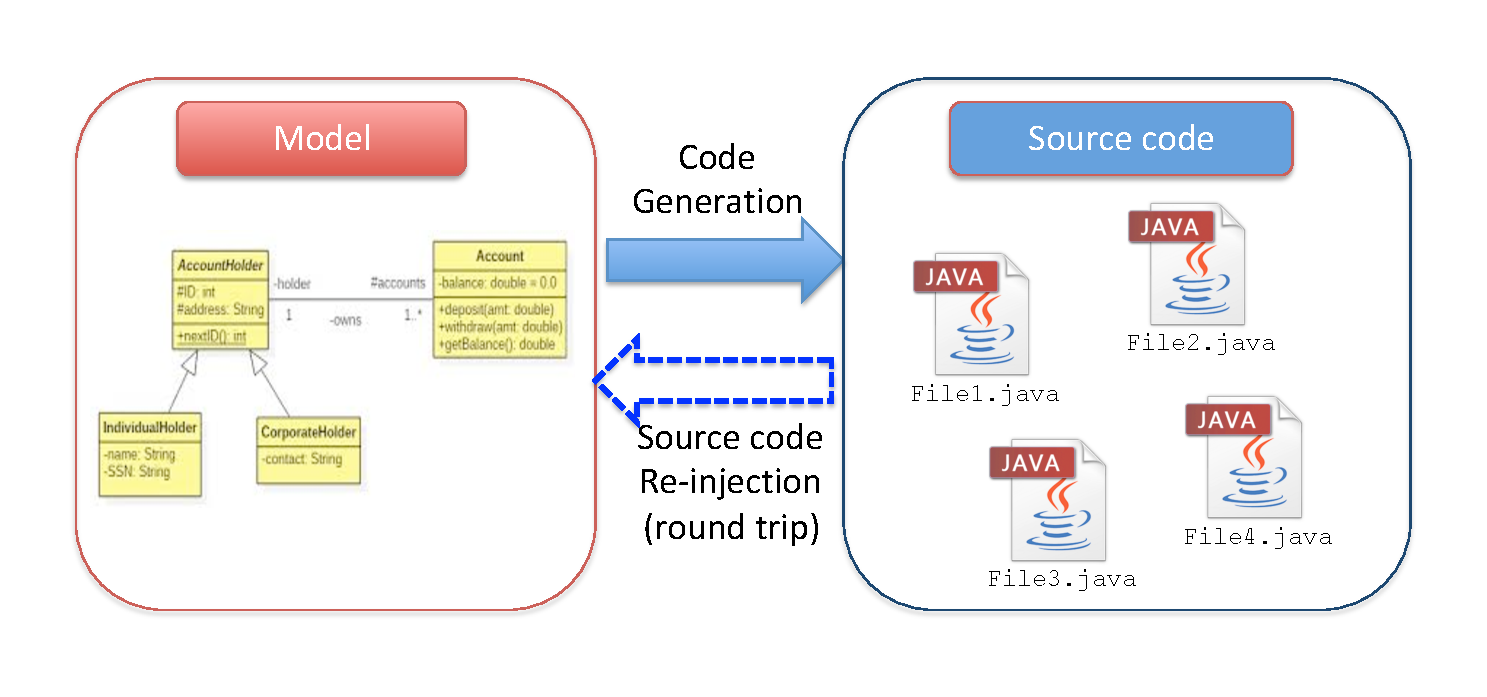
\includegraphics[width=1.0 \columnwidth]{ClassicalVision.pdf}
    \caption{Classical vision for Model-Driven Engineering}
    \label{fig:ClassicalVision}
\end{figure}


% Challenges description

This paper’s contributions are: ...

% Contributions

This paper is structured as follows: The second section focuses on .... 

% Plan de l'article
